\documentclass{beamer}
\usetheme{CambridgeUS}
\setbeamercolor{block title}{bg=red!80!black, fg=white}
\setbeamercolor{block body}{bg=red!10, fg=black}
%%%%%%%%%%%%%%%%%%%%%%%%%%%%%%%%%%%%%%%%%%%%%%%%%%%%%%%
\usepackage[utf8]{vietnam}
\usepackage{graphicx}
\usepackage{hyperref}
\usepackage{lipsum}
\usepackage{tikz}

\usepackage{bookmark}
\usepackage{amsmath}
\usepackage{amssymb}
%%%%%%%%%%%%%%%%%%%%%%%%%%%%%%%%%%%%%%%%%%%%%%%%%%%%%%%
% \AtBeginSection[]
% {
% \begin{frame}<beamer>
% \frametitle{Nội dung}

% \tableofcontents[
% currentsection,
% subsectionstyle=hide/hide,
% subsubsectionstyle=hide/hide
%]

% \end{frame}
%}
%%%%%%%%%%%%%%%%%%%%%%%%%%%%%%%%%%%%%%%%%%%%%%%%%%%%%%%
% \title[{\makebox[.15\paperwidth]{MI4100 - Mật mã và độ phức tạp thuật toán}}]{Chủ đề: Mô phỏng tấn công hệ mật mã khóa công khai RSA bằng thuật toán LLL giảm lưới}
% \author[Nhóm 8]{Nhóm 8}
% \date[\today]{\today}
%%%%%%%%%%%%%%%%%%%%%%%%%%%%%%%%%%%%%%%%%%%%%%%%%%%%%%%
\begin{document}
%%%%%%%%%%%%%%%%%%%%%%%%%%%%%%%%%%%%%%%%%%%%%%%%%%%%%%%
% % Trang tiêu đề
% % Cần có hình ảnh pictures/HUST2.jpeg
% % Không chỉnh sửa gì
% \begin{frame}
% \begin{tikzpicture}[remember picture, overlay]
% \node[anchor=center, inner sep=0pt] at (current page.center) {
\includegraphics[width=\paperwidth, height=\paperheight]{pictures/HUST2.jpeg}};
% \fill[white, opacity=0.8] (current page.south west) rectangle (current page.north east);
% \end{tikzpicture}
% \titlepage
% \end{frame}
%%%%%%%%%%%%%%%%%%%%%%%%%%%%%%%%%%%%%%%%%%%%%%%%%%%%%%%
% \begin{frame}{Danh sách thành viên}
% \begin{block}{Nhóm 8}
% \centering
% \begin{tabular} {|l|c|}
% \hline
% Họ và tên & MSSV \\
% \hline
% Vũ Văn Nghĩa & 20206205 \\
% Vũ Văn Nghĩa & 20206205 \\
% Vũ Văn Nghĩa & 20206205 \\
% Vũ Văn Nghĩa & 20206205 \\
% Vũ Văn Nghĩa & 20206205 \\
% \hline
% \end{tabular}
% \end{block}
% \end{frame}
%%%%%%%%%%%%%%%%%%%%%%%%%%%%%%%%%%%%%%%%%%%%%%%%%%%%%%%
% \begin{frame}{Phân công thành viên}
% \begin{block}{Phân công}
% \begin{itemize}
% \item Vũ Văn Nghĩa: Lập kế hoạch, phân chia công việc
% \item Vũ Văn Nghĩa: Lập kế hoạch, phân chia công việc
% \item Vũ Văn Nghĩa: Lập kế hoạch, phân chia công việc
% \item Vũ Văn Nghĩa: Lập kế hoạch, phân chia công việc
% \item Vũ Văn Nghĩa: Lập kế hoạch, phân chia công việc
% \end{itemize}
% \end{block}
% \end{frame}
%%%%%%%%%%%%%%%%%%%%%%%%%%%%%%%%%%%%%%%%%%%%%%%%%%%%%%%
%! %%%%%%%%%%%%%%%%%%%%%%%%%%%%%%%%%%%%%%%%%%%%%%%%%%%%%%
%! %%%%%%%%%%%%%%%%%%%%%%%%%%%%%%%%%%%%%%%%%%%%%%%%%%%%%%
%! %%%%%%%%%%%%%%%%%%%%%%%%%%%%%%%%%%%%%%%%%%%%%%%%%%%%%%
%! %%%%%%%%%%%%%%%%%%%%%%%%%%%%%%%%%%%%%%%%%%%%%%%%%%%%%%
%! %%%%%%%%%%%%%%%%%%%%%%%%%%%%%%%%%%%%%%%%%%%%%%%%%%%%%%
% \section{Tổng quan về hệ mật mã khóa công khai}
% \subsection{Lịch sử}
% \begin{frame}{Lịch sử}

% \begin{itemize}
% \item Hệ mật mã khóa công khai là một bước tiến lớn và là cuộc cách mạng trong lĩnh vực mật mã
% \item Hệ mật mã khóa công khai được Diffie và Hellman đưa ra năm 1976
% \end{itemize}

% \begin{columns}

% \begin{column}{0.4\textwidth}
% \begin{figure}[H]
% \centering
% 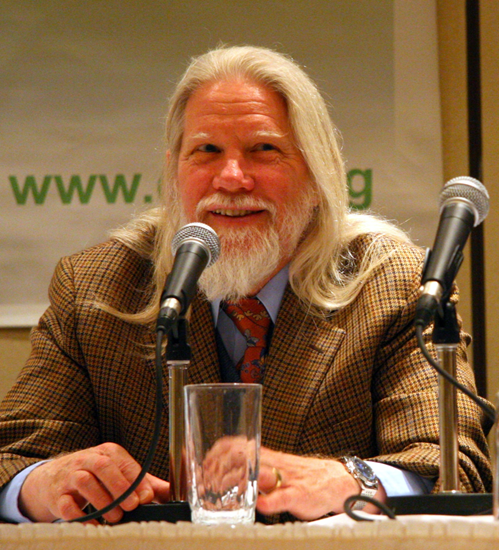
\includegraphics[scale = 0.4]{pictures/Bailey_Whitfield_Diffie.png}
% \end{figure}
% Bailey Whitfield 'Whit' Diffie\\ (sinh 05/06/1944 – 80 tuổi)
% \end{column}

% \begin{column}{0.4\textwidth}
% \begin{figure}[H]
% \centering
% 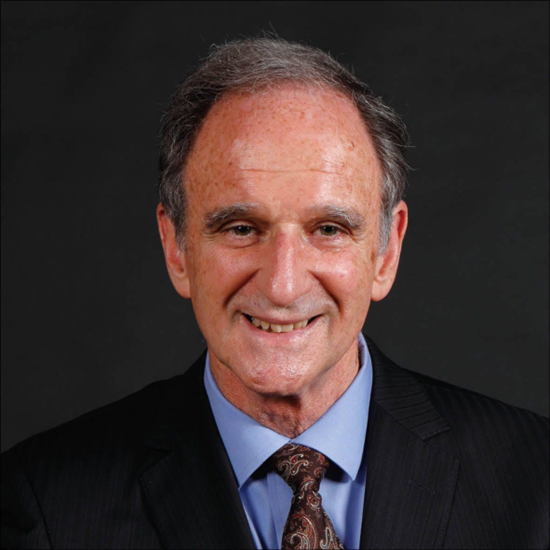
\includegraphics[scale = 0.4]{pictures/Martin_Edward_Hellman.png}
% \end{figure}
% Martin Edward Hellman\\(sinh 02/10/1945 - 79 tuổi)
% \end{column}

% \end{columns}
% \end{frame}
%%%%%%%%%%%%%%%%%%%%%%%%%%%%%%%%%%%%%%%%%%%%%%%%%%%%%%%
% \subsection{Khái niệm}
% \begin{frame}{Khái niệm}

% \begin{itemize}
% \item Hệ mật mã khóa công khai là một dạng mật mã hoá cho phép người sử dụng trao đổi các thông tin mật mà không cần phải trao đổi các khoá chung bí mật trước đó
% \item Việc mã hóa công khai được thực hiện bằng cách sử dụng một cặp khóa có quan hệ toán học với nhau là khóa công khai và khoá bí mật
% \begin{itemize}
% \item Khóa công khai: được công khai phổ biến - dùng để mã hóa
% \item Khóa bí mật: được giữ bí mật - dùng để giải mã
% \end{itemize}
% \end{itemize}

% $\Rightarrow$ Điều này đảm bảo hệ thống là không thể (hoặc rất khó) tìm ra khóa bí mật nếu chỉ biết khóa công khai

% \end{frame}
%%%%%%%%%%%%%%%%%%%%%%%%%%%%%%%%%%%%%%%%%%%%%%%%%%%%%%%
% \subsection{Mô hình tổng quát}
% \begin{frame}{Mô hình tổng quát}
% \begin{figure}[H]
% \centering
% 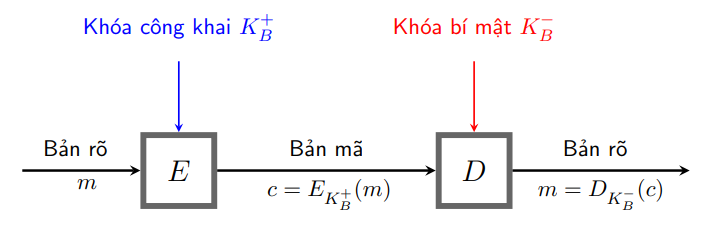
\includegraphics[scale = 0.6]{pictures/mo_hinh_tong_quat.png}
% \end{figure}

% \begin{block}{Nhận xét}
% Hệ mật mã khóa công khai là hệ mật mã bất đối xứng vì mã hóa và giải mã sử dụng khóa khác nhau
% \end{block}
% \end{frame}
%%%%%%%%%%%%%%%%%%%%%%%%%%%%%%%%%%%%%%%%%%%%%%%%%%%%%%%
% \subsection{Ưu, nhược điểm của hệ mã hóa công khai}
% \begin{frame}{Ưu, nhược điểm của hệ mã hóa công khai}
% \begin{block}{Ưu điểm}
% \begin{itemize}
% \item Thuật toán được viết một lần, công khai cho nhiều lần dùng, cho nhiều người dùng, họ chỉ cần giữ bí mật khóa riêng của mình
% \item Khi biết các tham số ban đầu của hệ mã hóa, việc tính ra cặp khoá công khai và bí mật phải là "dễ", tức là trong thời gian đa thức
% \item Khả năng lộ khóa bí mật khó hơn vì chỉ có một người giữ gìn. Nếu thám mã biết khoá công khai, cố gắng tìm khoá bí mật, thì chúng phải đương đầu với bài toán "khó"
% \item Nếu thám mã biết khoá công khai và bản mã, thì việc tìm ra bản rõ cũng là bài toán "khó"
% \end{itemize}
% \end{block}
% \end{frame}
%%%%%%%%%%%%%%%%%%%%%%%%%%%%%%%%%%%%%%%%%%%%%%%%%%%%%%%
% \begin{frame}{Ưu, nhược điểm của hệ mã hóa công khai}
% \begin{block}{Nhược điểm}
% \begin{itemize}
% \item Hệ mã hóa khóa công khai: mã hóa và giải mã chậm hơn hệ mã hóa khóa bí mật
% \item Khả năng bị tấn công dạng tấn công người đứng giữa do kẻ tấn công lợi dụng việc phân phối khóa công khai để thay giả mạo gói tin
% \end{itemize}
% \end{block}
% \end{frame}
%%%%%%%%%%%%%%%%%%%%%%%%%%%%%%%%%%%%%%%%%%%%%%%%%%%%%%%

%! %%%%%%%%%%%%%%%%%%%%%%%%%%%%%%%%%%%%%%%%%%%%%%%%%%%%%%
%! %%%%%%%%%%%%%%%%%%%%%%%%%%%%%%%%%%%%%%%%%%%%%%%%%%%%%%
%! %%%%%%%%%%%%%%%%%%%%%%%%%%%%%%%%%%%%%%%%%%%%%%%%%%%%%%
%! %%%%%%%%%%%%%%%%%%%%%%%%%%%%%%%%%%%%%%%%%%%%%%%%%%%%%%
%! %%%%%%%%%%%%%%%%%%%%%%%%%%%%%%%%%%%%%%%%%%%%%%%%%%%%%%
% \section{Hệ mật mã RSA}
% \subsection{Tổng quan về hệ mật mã RSA}
% \begin{frame}{Tổng quan về hệ mật mã RSA}

% \begin{itemize}
% \item RSA là hệ mật mã khóa công khai phổ biến và cũng đa năng nhất trong thực tế, phát minh bởi Rivest, Shamir và Adleman (1977)
% \item Cơ sở thuật toán RSA dựa trên tính khó của bài toán phân tích các số lớn ra thừa số nguyên tố: không tồn tại thuật toán thời gian đa thức (theo độ dài của biểu diễn nhị phân của số đó) cho bài toán này.
% \end{itemize}

% \begin{figure}[H]
% \centering
% 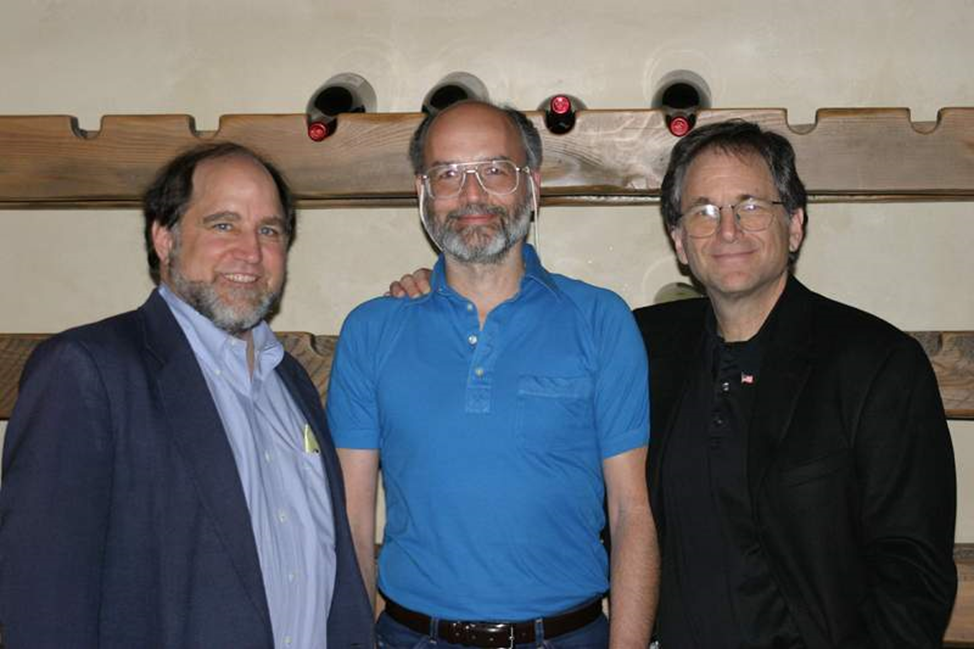
\includegraphics[scale = 0.4]{pictures/RSA_RonRivestAdiShamirLeonardAdleman.png}
% \end{figure}

% \end{frame}
%%%%%%%%%%%%%%%%%%%%%%%%%%%%%%%%%%%%%%%%%%%%%%%%%%%%%%%
% \subsection{Mã hóa và giải mã RSA}
% \begin{frame}{Mã hóa và giải mã RSA}
% \begin{itemize}
% \item Bảo mật của RSA dựa trên giả thuyết không có các thuật toán đủ nhanh để khai triển luỹ thừa một số. Qui trình áp dụng RSA gồm hai bước:
% \begin{enumerate}
% \item Lựa chọn (sinh) cặp khóa công khai và khóa bí mật
% \item Thực hiện thuật toán mã hoá và thuật toán giải mã
% \end{enumerate}
% \end{itemize}
% \end{frame}
%%%%%%%%%%%%%%%%%%%%%%%%%%%%%%%%%%%%%%%%%%%%%%%%%%%%%%%
% \begin{frame}{Mã hóa và giải mã RSA}
% \begin{itemize}
% \item Thuật toán sinh khóa

% \begin{enumerate}
% \item Chọn hai số nguyên tố đủ lớn, $p$ và $q$
% \item Tính toán $n = pq$ và $\phi(n) = (p - 1)(q - 1)$
% \item Chọn một số, $e$ $(1 < e < \phi(n))$ sao cho $\text{gcd}(e, \phi(n)) = 1$.

% Giá trị $e$ sẽ được sử dụng trong mã hoá
% \item Tìm một số $d$ sao cho $ed - 1$ chia hết cho $\phi(n)$, hay nói cách khác $d = e^{-1} \mod \phi(n)$. Giá trị $d$ sẽ được sử dụng để giải mã
% \item Công khai khóa $K^+_B$ = (n, e) và giữ bí mật khóa $K^-_B$ = (n, d)
% \end{enumerate}
% \end{itemize}
% \end{frame}
%%%%%%%%%%%%%%%%%%%%%%%%%%%%%%%%%%%%%%%%%%%%%%%%%%%%%%%
% \begin{frame}{Mã hóa và giải mã RSA}
% \begin{itemize}
% \item Mã hóa:

% \[
% c = E (m, K_B^+) = m^e \mod n
% \]
% \item Giải mã:

% \[
% m = D (c, K_B^-) = c^d \mod n
% \]
% \end{itemize}
% \end{frame}
%%%%%%%%%%%%%%%%%%%%%%%%%%%%%%%%%%%%%%%%%%%%%%%%%%%%%%%
% \begin{frame}{Ví dụ về RSA}
% \begin{block}{Ví dụ}
% Cho bản rõ \(M = 15 \) sử dụng thuật toán RSA với \(p = 11 \), \(q = 3 \), và \(e = 3 \)
% \end{block}

% \begin{itemize}
% \item Thuật toán sinh khóa

% \begin{enumerate}
% \item[Bước 1] \textbf{Với hai số nguyên tố}: $p = 11, \quad q = 3 \quad \Rightarrow \quad n = p \cdot q = 11 \cdot 3 = 33$
% \item[Bước 2] \textbf{Tính hàm Euler}:
% \[
% \varphi(n) = (p - 1) \cdot (q - 1) = (11 - 1) \cdot (3 - 1) = 10 \cdot 2 = 20
% \]
% \item[Bước 3] \textbf{Với số $e = 3$ nguyên tố cùng nhau với $\varphi(n) = 20$}:
% \item[Bước 4] \textbf{Tính $d$ là nghịch đảo của $e$ trong modulo $\varphi(n)$}:
% \[
% d \cdot e \equiv 1 \pmod{20}
% \]
% Ta có:
% \[
% d \cdot 3 \equiv 1 \pmod{20} \quad \Rightarrow \quad d = 7 \quad \text{(theo thuật toán Euclid)}
% \]
% \end{enumerate}

% \end{itemize}
% \end{frame}
%%%%%%%%%%%%%%%%%%%%%%%%%%%%%%%%%%%%%%%%%%%%%%%%%%%%%%%
% \begin{frame}{Ví dụ về RSA}
% \begin{itemize}
% \item Thuật toán sinh khóa

% \begin{enumerate}
% \item[Bước 5] \textbf{Khóa công khai và khóa bí mật}:
% \begin{itemize}
% \item \textbf{Khóa công khai} $(K_B^+)$:
% \[
% (n, e) = (33, 3)
% \]
% \item \textbf{Khóa bí mật} $(K_B^-)$:
% \[
% (n, d) = (33, 7)
% \]
% \end{itemize}
% \end{enumerate}
% \end{itemize}
% \end{frame}
%%%%%%%%%%%%%%%%%%%%%%%%%%%%%%%%%%%%%%%%%%%%%%%%%%%%%%%
% \begin{frame}{Ví dụ về RSA}

% \begin{itemize}

% \item \textbf{Mã hóa bản rõ $M = 15$}:
% \[
% C = M^e \mod n = 15^3 \mod 33
% \]
% Tính toán:
% $15^3 = 3375 \Rightarrow C = 9$

% \item \textbf{Giải mã bản mã $C = 9$}:
% \[
% M = C^d \mod n = 9^7 \mod 33
% \]
% Tính toán:
% \[
% 9^2 = 81 \quad \Rightarrow \quad 81 \mod 33 = 15
% \]
% \[
% 9^4 = 15^2 = 225 \quad \Rightarrow \quad 225 \mod 33 = 24
% \]
% \[
% 9^7 = 9^{4+2+1} = 9^4 \cdot 9^2 \cdot 9 = 24 \cdot 15 \cdot 9 = 3240 \quad \Rightarrow \quad 3240 \mod 33 = 15
% \]
% \[
% \Rightarrow M = 15
% \]

% \end{itemize}
% \end{frame}
%%%%%%%%%%%%%%%%%%%%%%%%%%%%%%%%%%%%%%%%%%%%%%%%%%%%%%%
% \begin{frame}{Ví dụ về RSA}

% \begin{itemize}

% \item Lập trình

% \begin{figure}[H]
% \centering
% 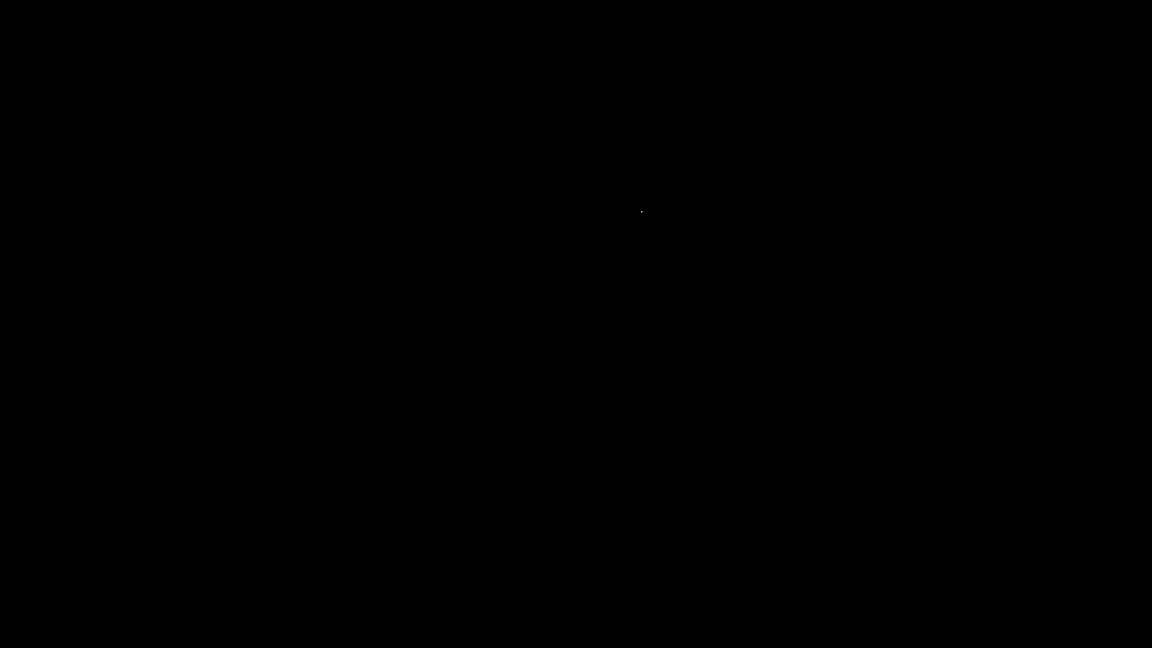
\includegraphics[scale = 0.15]{pictures/black.png}
% \end{figure}

% \end{itemize}
% \end{frame}
%%%%%%%%%%%%%%%%%%%%%%%%%%%%%%%%%%%%%%%%%%%%%%%%%%%%%%%

%! %%%%%%%%%%%%%%%%%%%%%%%%%%%%%%%%%%%%%%%%%%%%%%%%%%%%%%
%! %%%%%%%%%%%%%%%%%%%%%%%%%%%%%%%%%%%%%%%%%%%%%%%%%%%%%%
%! %%%%%%%%%%%%%%%%%%%%%%%%%%%%%%%%%%%%%%%%%%%%%%%%%%%%%%
%! %%%%%%%%%%%%%%%%%%%%%%%%%%%%%%%%%%%%%%%%%%%%%%%%%%%%%%
%! %%%%%%%%%%%%%%%%%%%%%%%%%%%%%%%%%%%%%%%%%%%%%%%%%%%%%%
% \section{Lý thuyết lưới}
% \begin{frame}{Lý thuyết lưới}
% \begin{itemize}
% \item Lý thuyết lưới là một lĩnh vực trong toán học có liên quan đến việc nghiên cứu các cấu trúc đại số và hình học của các mạng lưới được phát triển từ những năm 1940.
% \item Lý thuyết lưới được sử dụng trong nhiều lĩnh vực:
% \begin{itemize}
% \item Lĩnh vực mật mã học
% \item Lĩnh vực khoa học máy tính
% \item Lĩnh vực kỹ thuật thông tin
% \end{itemize}
% \end{itemize}
% \end{frame}
%%%%%%%%%%%%%%%%%%%%%%%%%%%%%%%%%%%%%%%%%%%%%%%%%%%%%%%
% \subsection{Định nghĩa}
% \begin{frame}{Định nghĩa}
% \begin{block}{Tập hợp các vector độc lập tuyến tính}
% Tập hợp các vector \(\{x_1, x_2, \ldots, x_n\}\) trong \(\mathbb{R}^n\) độc lập tuyến tính nếu:
% \[
% c_1 x_1 + c_2 x_2 + \ldots + c_n x_n = 0 \text{với} c_i \in \mathbb{R}
% \]
% Dấu "=" xảy ra khi và chỉ khi \(c_1 = c_2 = \ldots = c_n = 0 \).
% \end{block}
% \end{frame}
%%%%%%%%%%%%%%%%%%%%%%%%%%%%%%%%%%%%%%%%%%%%%%%%%%%%%%%
% \begin{frame}{Định nghĩa}
% \begin{block}{Cơ sở của không gian vector}
% Cho \(n \geq 1 \), \(\{x_1, x_2, \ldots, x_n\}\) là một cơ sở của \(\mathbb{R}^n\). Lưới \(n \) chiều với cơ sở \(\{x_1, x_2, \ldots, x_n\}\) là tập hợp \(L \) tất cả các tổ hợp tuyến tính của các vector cơ sở đó với hệ số nguyên:
% \[
% L = \{a_1 x_1 + a_2 x_2 + \ldots + a_n x_n \mid a_i \in \mathbb{Z} \}
% \]
% Các vector \(\{x_1, x_2, \ldots, x_n\}\) được gọi là cơ sở của lưới.
% \end{block}
% \end{frame}
%%%%%%%%%%%%%%%%%%%%%%%%%%%%%%%%%%%%%%%%%%%%%%%%%%%%%%%
% \subsection{Bổ đề}
% \begin{frame}{Bổ đề}
% \begin{block}{Bổ đề}
% Cho $x_1, x_2, \ldots, x_n$ và $y_1, y_2, \ldots, y_n$ là hai cơ sở của lưới $L \subset \mathbb{R}^n$. Lấy $X$, $Y$ lần lượt là các ma trận $n \times n$ nhận $x_i$ (tương ứng $y_i$) là các hàng thứ $i$. Khi đó $Y = CX$ với $C$ là ma trận vuông $n \times n$ với các hệ số nguyên và $\det(C) = \pm 1$.
% \end{block}
% \end{frame}
%%%%%%%%%%%%%%%%%%%%%%%%%%%%%%%%%%%%%%%%%%%%%%%%%%%%%%%
% \begin{frame}{Chứng minh}
% Với mọi $y_i$ thuộc lưới với cơ sở $x_1, x_2, \ldots, x_n$ và mọi $x_i$ thuộc lưới với cơ sở $y_1, y_2, \ldots, y_n$. Khi đó:
% \[
% x_i = \sum_{j=1}^n b_{ij} y_j, \quad y_i = \sum_{j=1}^n c_{ij} x_j.
% \]

% Ta có thể viết gọn lại dưới dạng ma trận:
% \[
% X = BY, \quad Y = CX.
% \]

% Vì vậy ta có $X = BCX$ và $Y = CBY$. Do $x_1, x_2, \ldots, x_n$ và $y_1, y_2, \ldots, y_n$ là cơ sở trong không gian $\mathbb{R}^n$ nên ma trận $X$, $Y$ là ma trận khả nghịch.

% Suy ra $BC = CB = I$ và $\det(B) \det(C) = 1$. Thêm nữa, $B$, $C$ là các ma trận hệ số nguyên. Do đó:
% \[
% \begin{cases}
% \det(B) = \det(C) = 1, \\
% \det(B) = \det(C) = -1.
% \end{cases}
% \]
% \end{frame}
%%%%%%%%%%%%%%%%%%%%%%%%%%%%%%%%%%%%%%%%%%%%%%%%%%%%%%%
% \subsection{Nhận xét}
% \begin{frame}{Nhận xét}
% \begin{block}{Nhận xét}
% Định thức của một lưới không phụ thuộc vào cách chọn cơ sở.
% \end{block}

% \textbf{Chứng minh:}

% Giả sử lưới $L \subset \mathbb{R}^n$ có hai cơ sở $x_1, x_2, \ldots, x_n$ và $y_1, y_2, \ldots, y_n$. Theo Bổ đề ta có:
% \[
% |\det(Y)| = |\det(CX)| = |\det(C) \cdot \det(X)| = |\pm 1 \cdot \det(X)| = |\det(X)|
% \]

% \textbf{Ví dụ:} Đặt $\{x_1, x_2\}$ là cơ sở của lưới $L$. Với $x_1 = (1, 0)$, $x_2 = (0, 1)$. Khi đó:
% \[
% L = a_1 x_1 + a_2 x_2 \quad \text{với} \quad a_1, a_2 \in \mathbb{Z}
% \]

% Đặt:
% \[
% \begin{cases}
% y_1 = x_1 + 5x_2 = (1, 5) \\
% y_2 = x_2 = (0, 1)
% \end{cases}
% \]

% Suy ra $\{y_1, y_2\}$ là một cơ sở khác của lưới.

% \end{frame}
%%%%%%%%%%%%%%%%%%%%%%%%%%%%%%%%%%%%%%%%%%%%%%%%%%%%%%%
% \subsection{Trực giao hóa Gram-Schmidt}
% \begin{frame}{Trực giao hóa Gram-Schmidt}
% \begin{itemize}
% \item Phần này trình bày thuật toán Gram-Schmidt cổ điển cho việc chuyển một cơ sở bất kỳ trong $\mathbb{R}^n$ thành một cơ sở trực giao.
% \item Đây là kỹ thuật quan trọng trong thuật toán LLL.
% \end{itemize}
% \end{frame}
%%%%%%%%%%%%%%%%%%%%%%%%%%%%%%%%%%%%%%%%%%%%%%%%%%%%%%%
% \begin{frame}{Trực giao hóa Gram-Schmidt}

% Cho $x_1, x_2, \ldots, x_n$ là một cơ sở trong $\mathbb{R}^n$. Trực giao hóa Gram-Schmidt của $x_1, x_2, \ldots, x_n$ là một cơ sở $x_1^*, x_2^*, \ldots, x_n^*$ được định nghĩa như sau:

% \begin{itemize}
% \item[(i)] $x_1 = x_1^*$,
% \item[(ii)] $x_i^* = x_i - \sum_{j=1}^{i-1} \mu_{ij} x_j^*$, \quad $2 \leq i \leq n$, \quad $\mu_{ij} = \frac{\langle x_i, x_j^* \rangle}{\langle x_j^*, x_j^* \rangle}$.
% \end{itemize}

% \begin{block}{Chú ý}
% Nếu $x_1, x_2, \ldots, x_n$ là một cơ sở của lưới $L$ thì sau khi trực giao hóa ta thu được các vector $x_1^*, x_2^*, \ldots, x_n^*$ có thể không nằm trong lưới $L$.
% \end{block}

% \end{frame}
%%%%%%%%%%%%%%%%%%%%%%%%%%%%%%%%%%%%%%%%%%%%%%%%%%%%%%%
% \begin{frame}{Trực giao hóa Gram-Schmidt}

% Nếu ta đặt $\mu_{ii} = 1$ và $\mu_{ij} = 0$ với $1 \leq i < j \leq n$, ta có thể viết lại dưới dạng ma trận:

% \[
% \underset{X}{\underbrace{\begin{pmatrix}
% x_1 \\
% x_2 \\
% \vdots \\
% x_n
% \end{pmatrix}}}
% =
% \underset{M}{\underbrace{\begin{pmatrix}
% 1 & 0 & \cdots & 0 \\
% \mu_{21} & 1 & \cdots & 0 \\
% \vdots & \vdots & \ddots & \vdots \\
% \mu_{n1} & \mu_{n2} & \cdots & 1
% \end{pmatrix}}}
% \underset{X^*}{\underbrace{\begin{pmatrix}
% x_1^* \\
% x_2^* \\
% \vdots \\
% x_n^*
% \end{pmatrix}}}
% \]

% \end{frame}
%%%%%%%%%%%%%%%%%%%%%%%%%%%%%%%%%%%%%%%%%%%%%%%%%%%%%%%
% \begin{frame}{Trực giao hóa Gram-Schmidt}

% Cho $x_1, x_2, \ldots, x_n$ là một cơ sở của $\mathbb{R}^n$ và $x_1^*, x_2^*, \ldots, x_n^*$ là trực giao hóa Gram-Schmidt của nó. Khi đó:

% \begin{itemize}
% \item[(i)] $\langle x_i^*, x_j^* \rangle = 0$ với $1 \leq i < j \leq n$,
% \item[(ii)] $\|x_k^*\| \leq \|x_k\|$,
% \item[(iii)] $\det(X^*) = \det(X)$.
% \end{itemize}

% \end{frame}
%%%%%%%%%%%%%%%%%%%%%%%%%%%%%%%%%%%%%%%%%%%%%%%%%%%%%%%
% \begin{frame}{Trực giao hóa Gram-Schmidt}

% \textbf{Chứng minh:}

% \begin{itemize}
% \item[(i)] Theo định nghĩa của quá trình trực giao hóa Gram-Schmidt, các vector $x_1^*, x_2^*, \ldots, x_n^*$ được xây dựng sao cho mỗi vector mới là trực giao với tất cả các vector trước đó. Cụ thể, với $x_i^*$ và $x_j^*$:
% \[
% x_j^* = x_j - \sum_{k=1}^{j-1} \mu_{jk} x_k^*, \quad \text{với} \quad \mu_{jk} = \frac{\langle x_j, x_k^* \rangle}{\langle x_k^*, x_k^* \rangle}
% \]
% Do đó, $ x_i^* x_j^* = 0$ với $1 \leq i < j \leq n$.
% \end{itemize}

% \end{frame}
%%%%%%%%%%%%%%%%%%%%%%%%%%%%%%%%%%%%%%%%%%%%%%%%%%%%%%%
% \begin{frame}{Trực giao hóa Gram-Schmidt}

% \textbf{Chứng minh:}

% \begin{itemize}
% \item[(ii)] Do $x_i^*$ là hình chiếu của $x_i$ lên không gian trực giao với các vector trước đó, ta có:
% \[
% x_i^* = x_i - \sum_{j=1}^{i-1} \mu_{ij} x_j^*
% \]

% Theo định lý Py-ta-go, ta có:

% \[
% \|x_k\|^2 = \|x_k^*\|^2 + \sum_{j=1}^{k-1} (\mu_{kj})^2 \|x_j^*\|^2.
% \]

% Do đó, $\|x_i^*\| \leq \|x_i\|$.
% \end{itemize}

% \end{frame}
%%%%%%%%%%%%%%%%%%%%%%%%%%%%%%%%%%%%%%%%%%%%%%%%%%%%%%%
% \begin{frame}{Trực giao hóa Gram-Schmidt}

% \textbf{Chứng minh:}

% \begin{itemize}
% \item[(iii)] Theo quá trình Gram-Schmidt, ta có $X = MX^*$ với $M$ là ma trận tam giác dưới với các phần tử đường chéo bằng 1 và các phần tử dưới đường chéo chính là các hệ số $\mu_{ij}$. Ma trận $M$ có định thức bằng 1, do đó:
% \[
% \det(X) = \det(MX^*) = \det(M) \det(X^*) = 1 \cdot \det(X^*) = \det(X^*)
% \]
% \end{itemize}

% \end{frame}
%%%%%%%%%%%%%%%%%%%%%%%%%%%%%%%%%%%%%%%%%%%%%%%%%%%%%%%
% \begin{frame}{Trực giao hóa Gram-Schmidt}

% Cho $x_1, x_2, \ldots, x_n$ là một cơ sở của $\mathbb{R}^n$ và $x_1^*, x_2^*, \ldots, x_n^*$ là trực giao hóa Gram-Schmidt của nó. Ta có:

% \[
% |\det(X)| \leq \|x_1\|\|x_2\|\cdots\|x_n\|.
% \]

% \textbf{Chứng minh:}

% Ta có $|\det(X^*)|$ là thể tích hình hộp $n$ chiều căng bởi các vector trực giao $x_1^*, x_2^*, \ldots, x_n^*$. Do đó:

% \[
% |\det(X^*)| = \|x_1^*\|\|x_2^*\|\cdots\|x_n^*\|.
% \]

% Theo Định lý 2.2, ta có:

% \[
% |\det(X)| = |\det(X^*)| \leq \|x_1^*\|\|x_2^*\|\cdots\|x_n^*\| \leq \|x_1\|\|x_2\|\cdots\|x_n\|.
% \]

% \end{frame}
%%%%%%%%%%%%%%%%%%%%%%%%%%%%%%%%%%%%%%%%%%%%%%%%%%%%%%%
% \section{Thuật toán LLL}
% \begin{frame}{Thuật toán LLL}
% \begin{itemize}
% \item Những ứng dụng của lý thuyết lưới trong hệ mật mã được phát triển từ khi có thuật toán rút gọn cơ sở lưới
% \item Thuật toán rút gọn cơ sở lưới do ba nhà toán học Arjen Lenstra, Hendrik Lenstra, László Lovász tìm ra (được viết tắt là LLL) năm 1982
% \item Ý tưởng của việc rút gọn cơ sở là thay đổi cơ sở $B$ của lưới $L$ thành một cơ sở mới $B'$ ngắn hơn sao cho $|\det(L)|$ không đổi.
% \end{itemize}
% \end{frame}
%%%%%%%%%%%%%%%%%%%%%%%%%%%%%%%%%%%%%%%%%%%%%%%%%%%%%%%
% \subsection{Giảm lưới 2 chiều}
% \begin{frame}{Giảm lưới 2 chiều}
% \begin{itemize}
% \item Việc giảm cơ sở lưới 2 chiều tương đối dễ hiểu.
% \item Đặt $\{x_1, x_2\}$ làm cơ sở của lưới 2 chiều.
% \item Mục tiêu của chúng ta sẽ thay thế cơ sở này bằng cơ sở giảm.
% \begin{enumerate}
% \item Nếu $\|x_1\| > \|x_2\|$ ta sẽ hoán vị $x_1$ với $x_2$.
% \item Thay vector $x_2$ bằng vector $x_2^*$ vuông góc với $x_1$ qua phép trực giao hóa Gram-Schmidt :
% $$x_2^* = x_2 - \frac{x_1.x_2}{x_1.x_1}.x_1 \text{.}$$ Đặt $t$ là số nguyên gần nhất với $\dfrac{x_1.x_2}{x_1.x_1}$
% \item Ta thay thế cơ sở $\{x_1, x_2 \}$ bằng cơ sở $$\{x_1, x_2 - tx_1\}\text{.}$$
% \item Lặp lại quy trình này đến khi không thể giảm cơ sở nữa.
% \end{enumerate}
% \end{itemize}
% \end{frame}
%%%%%%%%%%%%%%%%%%%%%%%%%%%%%%%%%%%%%%%%%%%%%%%%%%%%%%%
% \subsection{Cơ sở giảm}
% \begin{frame}{Cơ sở giảm}
% \begin{itemize}
% \item Một cơ sở $\{x_1, x_2\}$ được gọi là cơ sở giảm khi và chỉ khi
% \begin{enumerate}
% \item $\|x_1\| \leq \|x_2\|$,
% \item $|\mu| = \left|\dfrac{x_1.x_2}{x_1.x_1}\right| \leq \dfrac{1}{2}$.
% \end{enumerate}
% \end{itemize}

% \begin{block}{Ví dụ}
% Cho $\{x_1, x_2\}$ là cơ sở của lưới $L$ với $x_1 = (31, 59), x_2 = (37, 70)$. Thực hiện giảm cơ sở lưới trên.
% \end{block}

% \end{frame}
%%%%%%%%%%%%%%%%%%%%%%%%%%%%%%%%%%%%%%%%%%%%%%%%%%%%%%%
% \begin{frame}{Ví dụ}
% \begin{itemize}
% \item Ta thấy $\|x_1\| \leq \|x_2\|$. Ta có $\dfrac{x_1.x_2}{x_1.x_1} = \dfrac{5277}{4442} \approx 1, 18$\\

% Chọn $t_1 = 1 $ suy ra cơ sở mới: $$\begin{cases}
% x_1^{'} = x_1 = (31, 59)\\
% x_2^{'} = x_2 - t_1x_1 = (6, 11)
% \end{cases}$$
% \end{itemize}
% \end{frame}
%%%%%%%%%%%%%%%%%%%%%%%%%%%%%%%%%%%%%%%%%%%%%%%%%%%%%%%
% \begin{frame}{Ví dụ}
% \begin{itemize}
% \item Ta thấy $\|x_1'\| \geq \|x_2'\|$, hoán vị 2 vector ta có:
% $$\begin{cases}
% x_1^{'} = (6, 11)\\
% x_2^{'} = (31, 59)
% \end{cases} \text{.} $$

% \hspace*{1cm} Ta có: $\qquad \dfrac{x_1^{'}.x_2^{'}}{x_1^{'}.x_1^{'}} \approx 5, 3$\\
% + Chọn $t_2 = 5$ ta có cơ sở mới: $$\begin{cases}
% x_1^{''} = x_1^{'} = (6, 11) \\
% x_2^{''} = x_2^{'} - t_2x_1^{'} = (1, 4)
% \end{cases}$$
% \end{itemize}
% \end{frame}
%%%%%%%%%%%%%%%%%%%%%%%%%%%%%%%%%%%%%%%%%%%%%%%%%%%%%%%
% \begin{frame}{Ví dụ}
% \begin{itemize}
% \item Hoán vị vị trí $x_1^{''}$ và $x_2^{''}$ ta thu được cơ sở $$\begin{cases}
% x_1^{''}= (1, 4)\\
% x_2^{''}= (6, 11)
% \end{cases}$$
% \hspace*{1cm} Ta có $\dfrac{x_1^{''}.x_2^{''}}{x_1^{''}.x_1^{''}} = \dfrac{50}{17} \approx 2, 9$. \qquad Chọn $t_3 = 3$ ta có: $$\begin{cases}
% x_1^{(3)} = (1, 4)\\
% x_2^{(3)} = x_2^{''} - 3.x_1^{''} = (3, -1)
% \end{cases}$$\\

% \end{itemize}
% \end{frame}
%%%%%%%%%%%%%%%%%%%%%%%%%%%%%%%%%%%%%%%%%%%%%%%%%%%%%%%
% \begin{frame}{Ví dụ}
% \begin{itemize}
% \item Hoán vị 2 vector ta có $$\begin{cases}
% x_1^{(3)} = (3, -1)\\
% x_2^{(3)} = (1, 4)
% \end{cases}$$
% \hspace*{1cm}Ta thấy $\dfrac{x_1^{(3)}.x_2^{(3)}}{x_1^{(3)}.x_1^{(3)}} = -\dfrac{1}{10}$

% $\Rightarrow$ Suy ra $\{x_1^{(3)}, x_2^{(3)}\}$ là cơ sở giảm.\vspace{0.5cm}

% \end{itemize}
% \end{frame}
%%%%%%%%%%%%%%%%%%%%%%%%%%%%%%%%%%%%%%%%%%%%%%%%%%%%%%%
% \subsection{Định lý}
% \begin{frame}{Định lý}
% \begin{block}{Định lý}
% Nếu $x_1, x_2$ là cơ sở rút gọn của lưới $L$ thì $x_1$ là vector khác $0$ ngắn nhất của lưới đó.
% \end{block}

% Chứng minh.

% Đặt $ax_1 + bx_2$ là vector khác không bất kì trong lưới $L$ (với $a, b \in Z$).\\
% Ta có: \hspace{4cm}$ \quad \|ax_1 + bx_2\|^2 = a^2\|x_1\|^2 + b^2\|x_2\|^2 + 2abx_1x_2$\\
% Vì $x_1, x_2$ là cơ sở giảm nên: $$-\frac{1}{2}x_1x_1 \leq x_1x_2 \leq \frac{1}{2}x_1x_1 \text{.}$$
% Suy ra: \hspace{3cm} $\qquad 2abx_1x_2 \geq -|ab|\|x_1\|^2 $

% \end{frame}
%%%%%%%%%%%%%%%%%%%%%%%%%%%%%%%%%%%%%%%%%%%%%%%%%%%%%%%
% \begin{frame}{Định lý}

% Do đó
% $$
% \begin{aligned}
% \|ax_1 + bx_2\|^2 &\geq a^2\|x_1\|^2 - |ab|\|x_1\|^2 + b^2\|x_2\|^2 \\
% & \geq a^2\|x_1\|^2 - |ab|\|x_1\|^2 + b^2\|x_1\|^2 \quad (\text{do}\|x_2\| \geq \|x_1\|)\\
% & = (a^2 - |ab| + b^2) \|x_1\|^2 \text{.}
% \end{aligned}
% $$
% Ta thấy $a^2 - |ab| + b^2 \in N$ và bằng 0 khi và chỉ khi $a = b = 0$.\\
% Nhưng \quad $ax_1 + bx_2 \ne 0$ \qquad $\Rightarrow$ \qquad Trường hợp $a = b = 0$ (loại).\\
% \hspace*{3cm}$\Rightarrow a^2 - |ab| + b^2 \geq 1$\\
% \hspace*{3cm}$ \Rightarrow \|ax_1 + bx_2\| \geq \|x_1\|^2$.\\
% Do đó $x_1$ là vector khác $0$ ngắn nhất của lưới
% \end{frame}
%%%%%%%%%%%%%%%%%%%%%%%%%%%%%%%%%%%%%%%%%%%%%%%%%%%%%%%
% \subsection{Thuật toán giảm lưới 2 chiều}
% \begin{frame}{Thuật toán giảm lưới 2 chiều} 





% \begin{enumerate}
%     \item     Nhập vào cơ sở lưới 2 chiều ${b_1,b_2} \in R^2$.
%     \item     Nếu $\|b_1\| > \|b_2\|$, ta hoán đổi vị trí $b_1$ và $b_2$.
%     \item     Đặt $t$ bằng phần nguyên $\left|\dfrac{b_1.b_2}{b_1.b_1}\right|$. 

%     Nếu $t = 0$, dừng lại và kết luận là cơ sở giảm. 

%     Ngược lại, ta tính lại $b_2 = b_2 - t.b_1$ và quay lại bước 2 
% \end{enumerate}



% \end{frame}
%%%%%%%%%%%%%%%%%%%%%%%%%%%%%%%%%%%%%%%%%%%%%%%%%%%%%%%
% \begin{frame}{Thuật toán giảm lưới 2 chiều} 




% \begin{figure}[h!]
% \centering
%   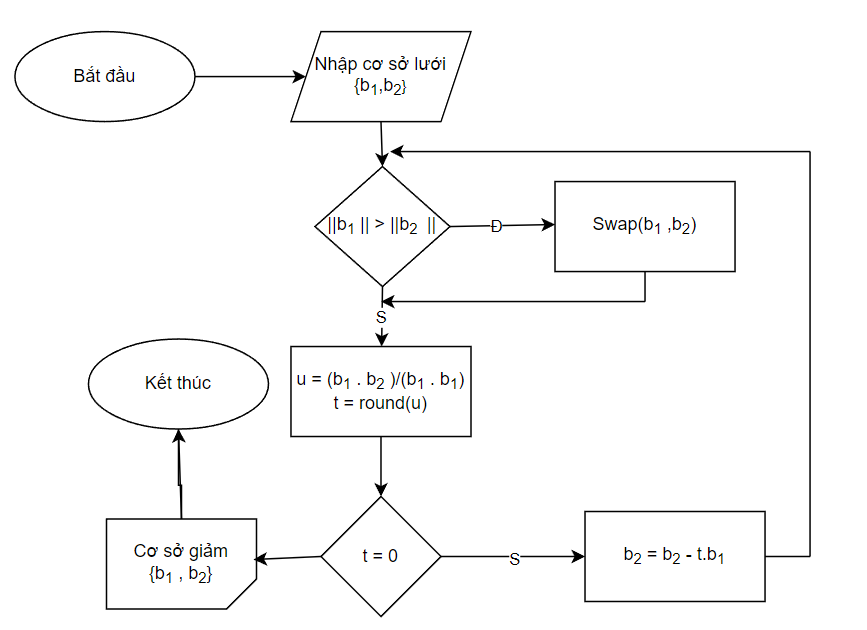
\includegraphics[scale = 0.6]{pictures/a.10.png}
%   \label{fig:boat1}
% \end{figure}



%     \end{frame}
%%%%%%%%%%%%%%%%%%%%%%%%%%%%%%%%%%%%%%%%%%%%%%%%%%%%%%%
% \subsection{Giảm lưới nhiều chiều}
% \begin{frame}{Giảm lưới nhiều chiều}
%     \begin{itemize}
%         \item Việc giảm cơ sở lưới nhiều    chiều  khó khăn hơn nhiều
%         \item   Thuật toán LLL  sử dụng cách tiếp cận tìm kiếm các vector gần như ngắn nhất(trong thời gian đa thức)
%     \end{itemize}
% \end{frame}
%%%%%%%%%%%%%%%%%%%%%%%%%%%%%%%%%%%%%%%%%%%%%%%%%%%%%%%
% \begin{frame}{Định nghĩa}
%     \begin{itemize}
%         \item Tham số rút gọn $\alpha$ là một số thực sao cho $\dfrac{1}{4} < \alpha < 1$. Giá trị chính tắc của $\alpha$ là $\alpha = \dfrac{3}{4}$
%         \item  Cơ sở $x_1,x_2,...,x_n$ được gọi là một cơ sở $\alpha$-rút gọn nếu nó thỏa mãn:
%               \begin{enumerate}
%                   \item $|\mu_{ij}| \leq \dfrac{1}{2} $ với $1 \leq j < i \leq n$,
%                   \item $\|x_i^*\|^2 \geq (\alpha - \mu_{i,i-1}^2)\|x_{i-1}^*\|^2$ với $2\leq i \leq n$.
%               \end{enumerate}
%         \item  Ta định nghĩa tham số bổ trợ  $\beta$ như sau: \quad $\beta = \dfrac{4}{4\alpha - 1}$
%     \end{itemize}
% \end{frame}
%%%%%%%%%%%%%%%%%%%%%%%%%%%%%%%%%%%%%%%%%%%%%%%%%%%%%%%
% \begin{frame}{Định nghĩa}
%     \begin{itemize}
%         \item   Nếu $x_1,x_2,...,x_n$ là một cơ sở $\alpha$-rút gọn của lưới $L$ trong $R^n$ và $x_1^*,x_2^*,...,x_n^*$ là cơ sở trực giao hóa Gram-Schmidt của nó thì:
%               \begin{enumerate}
%                   \item $\|x_j\|^2 \leq \beta^{i-1}\|x_i^*\|^2$ với $1 \leq j \leq i \leq n $,
%                   \item $\|x_1\|.\|x_2\|...\|x_n\| \leq \beta^{\tfrac{n(n-1)}{4}}det(L)$,
%                   \item $\|x_1\| \leq \beta^{\tfrac{(n-1)}{4}}det(L)^{\frac{1}{n}} $.
%               \end{enumerate}
%     \end{itemize}
% \end{frame}
%%%%%%%%%%%%%%%%%%%%%%%%%%%%%%%%%%%%%%%%%%%%%%%%%%%%%%%






%%%%%%%%%%%%%%%%%%%%%%%%%%%%%%%%%%%%%%%%%%%%%%%%%%%%%%%
% \section{Ứng dụng lý thuyết lưới trong hệ mật mã RSA}
% \begin{frame}{Ứng dụng lý thuyết lưới trong hệ mật mã RSA}
% \begin{itemize}
% \item
% \end{itemize}
% \end{frame}
%%%%%%%%%%%%%%%%%%%%%%%%%%%%%%%%%%%%%%%%%%%%%%%%%%%%%%%
% \section{Thực hiện chương trình}
% \begin{frame}{Thực hiện chương trình}
% % \begin{itemize}
% % 1 2 3 4
% % \end{itemize}

% % nền trắng
% \end{frame}
%%%%%%%%%%%%%%%%%%%%%%%%%%%%%%%%%%%%%%%%%%%%%%%%%%%%%%%
%! %%%%%%%%%%%%%%%%%%%%%%%%%%%%%%%%%%%%%%%%%%%%%%%%%%%%%%
%! %%%%%%%%%%%%%%%%%%%%%%%%%%%%%%%%%%%%%%%%%%%%%%%%%%%%%%
%! %%%%%%%%%%%%%%%%%%%%%%%%%%%%%%%%%%%%%%%%%%%%%%%%%%%%%%
%! %%%%%%%%%%%%%%%%%%%%%%%%%%%%%%%%%%%%%%%%%%%%%%%%%%%%%%
%! %%%%%%%%%%%%%%%%%%%%%%%%%%%%%%%%%%%%%%%%%%%%%%%%%%%%%%
% \section{Tổng kết}
% \subsection{Tổng kết}
% \subsubsection{Tổng kết}
% \begin{frame}{Tổng kết}
%
% Trên đây là toàn văn báo cáo Đồ án 1 về chủ đề \textbf{Phương pháp lưới}. Trong đồ án này, em đã trình bày một số kiến thức cơ bản về lý thuyết lưới, tìm hiểu về thuật toán LLL và nhận thấy một phần tầm quan trọng của nó tróng lý thuyết số và mật mã.Trong bài báo cáo có giới thiệu về một số hệ mật mã như RSA và NTRU, thực hiện các cuộc tấn công vào chúng và thực hiện chạy chương trình thực nghiệm trên phần mềm SageMath.\\

% Báo
% cáo Đồ án vẫn còn rất nhiều thiếu sót, vậy nên em rất mong được thầy và các bạn đọc cùng
% góp ý, nhận xét để báo cáo trở nên hoàn thiện hơn.\\

% \end{frame}
%%%%%%%%%%%%%%%%%%%%%%%%%%%%%%%%%%%%%%%%%%%%%%%%%%%%%%%

%! %%%%%%%%%%%%%%%%%%%%%%%%%%%%%%%%%%%%%%%%%%%%%%%%%%%%%%
%! %%%%%%%%%%%%%%%%%%%%%%%%%%%%%%%%%%%%%%%%%%%%%%%%%%%%%%
%! %%%%%%%%%%%%%%%%%%%%%%%%%%%%%%%%%%%%%%%%%%%%%%%%%%%%%%
%! %%%%%%%%%%%%%%%%%%%%%%%%%%%%%%%%%%%%%%%%%%%%%%%%%%%%%%
%! %%%%%%%%%%%%%%%%%%%%%%%%%%%%%%%%%%%%%%%%%%%%%%%%%%%%%%
% \section*{}
% \begin{frame}{}
% \centering
% \Huge{Thanks for listening!}
% \end{frame}
%%%%%%%%%%%%%%%%%%%%%%%%%%%%%%%%%%%%%%%%%%%%%%%%%%%%%%%
\end{document}

% <!-- !Đánh công thức toán tag -->
%